\documentclass[crop,tikz]{standalone}
\usetikzlibrary{positioning,arrows,fit,calc}
\pgfdeclarelayer{bg}
\pgfsetlayers{bg,main}
\tikzset{
	>=stealth'
}
\begin{document}
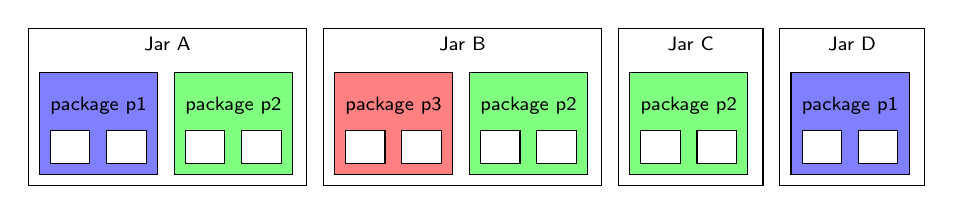
\begin{tikzpicture}[
node distance = 2mm,
every node/.style = {
	font = \sffamily\scriptsize
},
jar/.style = {
	draw,
	minimum height = 2.cm
},
package/.style = {
	draw,
	minimum height = 1.3cm,
	minimum width = 1.5cm
},
class/.style = {
	draw,
	fill = white,
	minimum height = \baselineskip,
	minimum width = .5cm
}
]

\node (jarA) [jar, text width = 33mm] {};
\node (jarA_t) [below] at (jarA.north) {Jar A};

\node (package_A1) [package, above right = of jarA.south west, fill=blue!50] {};
\node [below = of package_A1.north] {package p1};
\node (class_1) [class, above right = of package_A1.south west] {};
\node (class_2) [class, right = of class_1] {};

\node (package_A2) [package, right = of package_A1, fill=green!50] {};
\node [below = of package_A2.north] {package p2};
\node (class_3) [class, above right = of package_A2.south west] {};
\node (class_4) [class, right = of class_3] {};


\node (jarB) [jar, text width = 33mm, right = of jarA] {};
\node (jarB_t) [below] at (jarB.north) {Jar B};

\node (package_B3) [package, above right = of jarB.south west, fill=red!50] {};
\node [below = of package_B3.north] {package p3};
\node (class_5) [class, above right = of package_B3.south west] {};
\node (class_6) [class, right = of class_5] {};

\node (package_B2) [package, right = of package_B3, fill=green!50] {};
\node [below = of package_B2.north] {package p2};
\node (class_7) [class, above right = of package_B2.south west] {};
\node (class_8) [class, right = of class_7] {};

\node (jarC) [jar, right = of jarB, text width = 1.6cm] {};
\node (jarC_t) [below] at (jarC.north) {Jar C};

\node (package_C2) [package, above right = of jarC.south west, fill=green!50] {};
\node [below = of package_C2.north] {package p2};

\node (class_9) [class, above right = of package_C2.south west] {};
\node (class_10) [class, right = of class_9] {};

\node (jarD) [jar, right = of jarC, text width = 16mm] {};
\node (jarD_t) [below] at (jarD.north) {Jar D};


\node (package_D1) [package, above right = of jarD.south west, fill=blue!50] {};
\node [below = of package_D1.north] {package p1};
\node (class_11) [class, above right = of package_D1.south west] {};
\node (class_12) [class, right = of class_11] {};


\end{tikzpicture}

\end{document}